\documentclass[a4paper,10pt]{scrartcl}
\usepackage[utf8]{inputenc}
\usepackage[german]{babel}
\usepackage[top=3cm,bottom=3cm,right=3cm,left=3cm]{geometry}
\usepackage{graphicx}
\usepackage{listings}
\usepackage{color}
\usepackage{caption}
\usepackage{parskip}
%opening

\title{ECNF Zusammenfassung}
\author{Roland Hediger}
\renewcommand{\familydefault}{\sfdefault}

\definecolor{bluekeywords}{rgb}{0.13,0.13,1}
\definecolor{greencomments}{rgb}{0,0.5,0}
\definecolor{redstrings}{rgb}{0.9,0,0}

\lstset{language=[Sharp]C,numberstyle=\normalsize,
basicstyle=\footnotesize\ttfamily,
 numbers=left,               % Ort der Zeilennummern
 numberstyle=\tiny,          % Stil der Zeilennummern
 stepnumber=5,              % Abstand zwischen den Zeilennummern
 numbersep=5pt,              % Abstand der Nummern zum Text
 tabsize=2,                  % Groesse von Tabs
 extendedchars=true,         %
 breaklines=true,            % Zeilen werden Umgebrochen
 frame=b,         
 showspaces=false,           % Leerzeichen anzeigen ?
 showtabs=false,             % Tabs anzeigen ?
 xleftmargin=17pt,
 framexleftmargin=17pt,
 framexrightmargin=5pt,
 framexbottommargin=4pt,
 showstringspaces=false,    
escapeinside={(*@}{@*)},
commentstyle=\color{greencomments},
keywordstyle=\color{bluekeywords}\bfseries,
stringstyle=\color{redstrings},
}
\DeclareCaptionFont{white}{\color{white}}
\DeclareCaptionFormat{listing}{\colorbox{black}{\parbox{\textwidth}{#1#2#3}}}
\captionsetup[lstlisting]{format=listing,labelfont=white,textfont=white}
\newcommand{\pic}[2][Figure]{
  \begin{figure}[h!]
   \centering
   \includegraphics[scale=0.5]{#2}
   \caption{{#1}}
  \end{figure}
}

\begin{document}

\maketitle
\tableofcontents

\pagebreak
\section{Essenzielle Sachen}

\subsection{Feature Vergleich}

\begin{tabular}{|l|l|}
\hline
 \textbf{Wie in Java} & \textbf{Wie in C++} \\
 \hline
 Interfaces & Structs \\ \hline
 Exceptions & Operator Overloading \\ \hline
 Threading & Pointer arithmetic in unsicherer Code \\ \hline
 Namespaces & Manche syntaktische Details \\ \hline
 Starke Typisierung & Generics (\textit{Templates}) \\ \hline
 Garbage Collection & \\ \hline
 Reflektion & \\  \hline
 Dynamisches Laden von Code & \\ \hline
 Enums & \\ \hline
 Generics & \\ \hline
 Attributen & \\ \hline
 Annonyme Typen & \\ \hline
 foreach schleife & \\ \hline
\end{tabular}

\subsection{Echte Unterschiede}
\begin{tabular}{|p{7cm}|p{7cm}|}
\hline
 \textbf{Wirkliche Unterschiede} & \textbf{Syntaktische Zucker} \\ 
 \hline
  Call by Reference Parameter ( Stern in c++) & Properties \\ \hline
  Stack allozierte Objekten (structs werden auf Stack alloziert) & Events\\ \hline
  Block Matritzen & Delegates \\
  Uniform Typ System & Indexers (Indexoperator Überladung sozusagen)\\ \hline
  goto Anweisung & Boxing / Unboxing (Referenz in Value Typ  und umgekehrt)\\ \hline
  Versionierung & Statische Klassen \\ \hline
  Annonyme Methoden &  Partielle Klassen (über mehere Dateien zerlegt) \\ \hline
  Funktionale Programmierung & \\ \hline
  Native interoperabilität (Aufrufe von Methoden in anderen Sprachen (CLR) & \\ \hline
  Dynamische Programmierung & \\ \hline
  LINQ & \\ \hline
  \end{tabular}
\subsection{Typ Baum }
\begin{figure}[h]
 \centering
 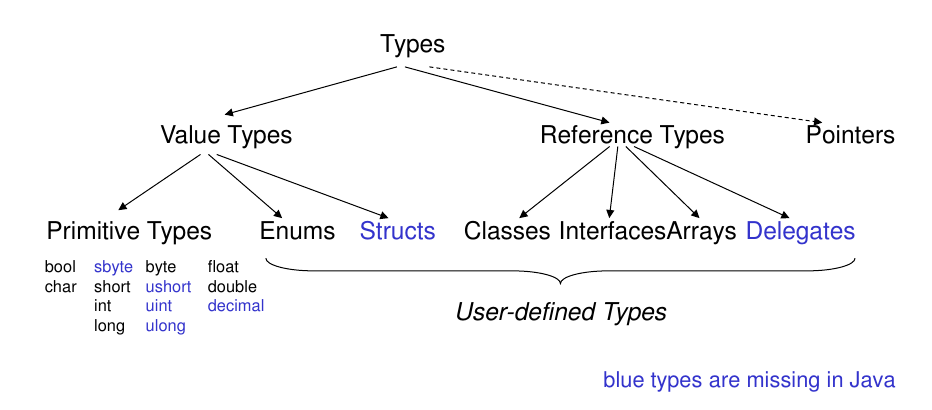
\includegraphics[scale=0.4]{./type_tree.png}
 % type_tree.png: 932x410 pixel, 96dpi, 24.66x10.85 cm, bb=0 0 699 307
 \caption{Typ Baum von c hash}
\end{figure}
\pagebreak
\subsection{Boxing and Unboxing}

\begin{lstlisting}[caption=Boxing und Unboxing]
 // boxing - Werttyp in Referenztyp umwandeln - Wert 3 ist jetzt in einem Heapobjekt geboxed
 object obj = 3;
 // Unboxing Referenztyp in Werttyp konvertieren durch casting.
 int x = (int) obj;
\end{lstlisting}

\subsection{Klassen}
\begin{lstlisting}[caption=Deklaration von eine Klasse]
class Hello {
private String name;
private void Greet() {...}
public static void Main(String[] args) {...}
}
\end{lstlisting}

\begin{description}
 \item [Statische Konstruktor] 1 mal per Typ ausgeführt, bevor alle instanzen oder andere statische mitglieder der Klasse 
 zugegriffen werden können. \textit{Bevor ist nicht klar wegen Intermidiate Language Übersetzung}
 \item[Statische Felder] werden bevor statische Konstruktor initializiert.
\end{description}

\subsection{Properties}
Properties sind syntaktische Zucker für Getter und Setter methoden. Die sind auch ein bisschen angenehmer.
Beispiel : \\
Das Property eliminiert die Methoden getFileName und setFileName. Stattdessen kann man das gleiche tun durch normallen zugriff mittels der Punkt :\\
data.FileName

\begin{lstlisting}[caption=Properties Beispiel]
//Deklaration
class Data {
string f;
public string FileName{ 
  set { f = value; }
  get { return f; }
  }
}
//Nutzung
Data d = new Data();
d.FileName = "myFile.txt";
string s = d.FileName;

// Teil 2 Automatische Properties
class Data {
public string FileName { get; set;}
}

\end{lstlisting}

\subsubsection{Automatische Properties}
Hier wird die private Variable vom System generiert im hintergrund (string f von oben), sowie auch der Inhalt von \texttt{get} und \texttt{set}\\
Es funktioniert genau gleich wie im ersten Teil des Beispiels

\subsection{C\# modifiers}

\textbf{Fields :}\\ \linebreak
\begin{tabular}{l | l}
\hline
Zugriff Modifiers & \texttt{public,internal,private,protected}\\
Statisch & \texttt{static}\\
Vererbung & \texttt{new} Selten benutzt. \\
Unsafe code & (pointers usw) \texttt{unsafe}\\
Read-only (final) & \texttt{readonly} \\
Threading & \texttt{volatile} \\
\hline
\end{tabular}

\textbf{Methoden :}\\ \linebreak
\begin{tabular}{l | l}
\hline
Zugriff Modifiers & \texttt{public,internal,private,protected}\\
Statisch & \texttt{static}\\
Vererbung & \texttt{new,virtual,orverride,abstract,sealed} \\
Unsafe unmanaged code & (pointers usw) \texttt{unsafe,extern}\\
\hline
\end{tabular}

\subsection{Indexers}

\begin{lstlisting}[caption=Indeexers]
 public class Portfolio
{
  Stock[] stocks;
  ...
  public Stock this[int index] // indexer impl{
  get { return this.stocks[index];}
  set { this.stocks[index] = value; }
}

Console.WriteLine(portfolio[i].Symbol);

\end{lstlisting}

\subsection{Abstract Classes}
\begin{lstlisting}[caption=Abstrakte Klassen]
 abstract class Stream {
public abstract void Write(char ch);
public void WriteString(string s) { foreach (char ch in s) Write(s); }
}
class File : Stream {
public override void Write(char ch) {... write ch to disk ...}
}

\end{lstlisting}
\pagebreak
\begin{enumerate}
 \item Abstrake Methoden sind nicht implementiert.
 \item Abstrakte Methoden sind implizit virtual.
  \subitem Definiton von Virtual :\\
  A virtual method can be redefined. The virtual keyword designates a method that is overridden in derived classes. We can add derived types without modifying the rest of the program. The runtime type of objects thus determines behavior.
  \item Falls eine Klasse abstrakte Methoden hat, die deklariert oder vererbt sind, muss die Klasse selbst abstrakt sein.
  \item Abstrakte klassen können nicht instanziert werden.
\end{enumerate}

\subsection{Interfaces}
\begin{lstlisting}[caption=Interface Beispiel]
 public interface IList : ICollection, IEnumerable {
int Add (object value);
 // methods
bool Contains (object value);
...
bool IsReadOnly { get; } // property
...
object this [int index] { get; set; }
//indexer
}


\end{lstlisting}

\begin{enumerate}
 \item Interface ist definiert so dass es in eine gewisse Art und Weise ähnlichkeiten mit C++ hat.
 \item Ein Interface ist eine rein abstrakte Klasse mit nur Methodensignaturen und keine implementationen.
 \item Es ist jedoch möglich dass ein Interface Methoden, Properties, sowie auch Indexers und Events beinhalten kann.
 \item Interface Mitglieder sind implizit public abstract (virtual).
 \item Interface Mitglieder mussen nicht statisch sein.
 \item Klasses sowohl als auch \textbf{Structs} können mehrere Interfaces implementieren.
 \item Interfaces könnnen andere Interfaces erweitern.
\end{enumerate}

\textbf{Klassen,Structs und Interfaces}

\begin{enumerate}
 \item Eine Klasse vererbt von einer einzigen Stamm/BaseKlasse. Es kann aber mehrere Interfaces implementieren.
 \item Ein Struct kann nicht von eine Stamm/Baseklasse (Typ) vererben. Es kann doch mehrere Interfaces implementieren.
 \item Alle Interface Methoden müssen implementiert werden.
 \item \textit{Interface methoden mussen keine \texttt{overrride} haben}
 \item Interface Methoden können als virtual oder abstrakt implementiert werden.
 \item Subclass override von Methoden = explizite  virtual Modifier.
\end{enumerate}
\pagebreak
\subsection{Standard Collections}
\begin{figure}[h]
 \centering
 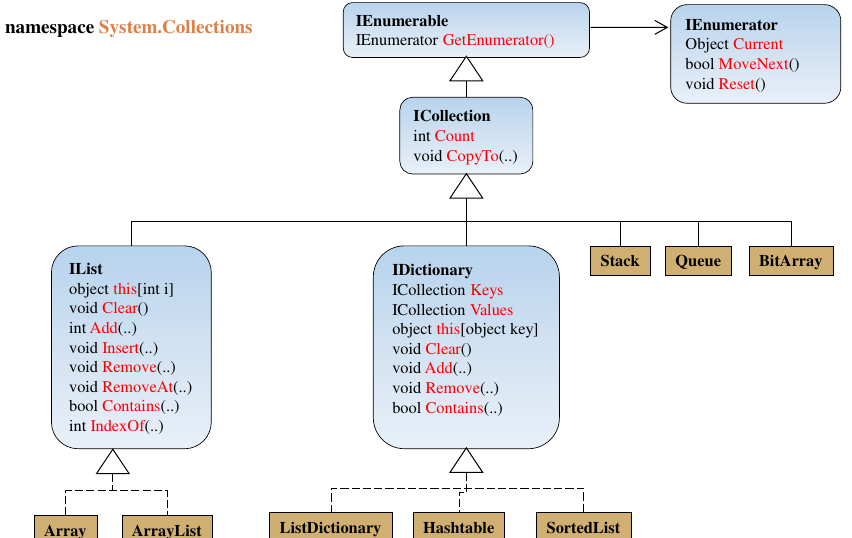
\includegraphics[scale=0.5]{./collections1.png}
 % collections1.png: 852x538 pixel, 96dpi, 22.54x14.23 cm, bb=0 0 639 403
 \caption{Standard Collections}
\end{figure}
\begin{figure}[h]
 \centering
 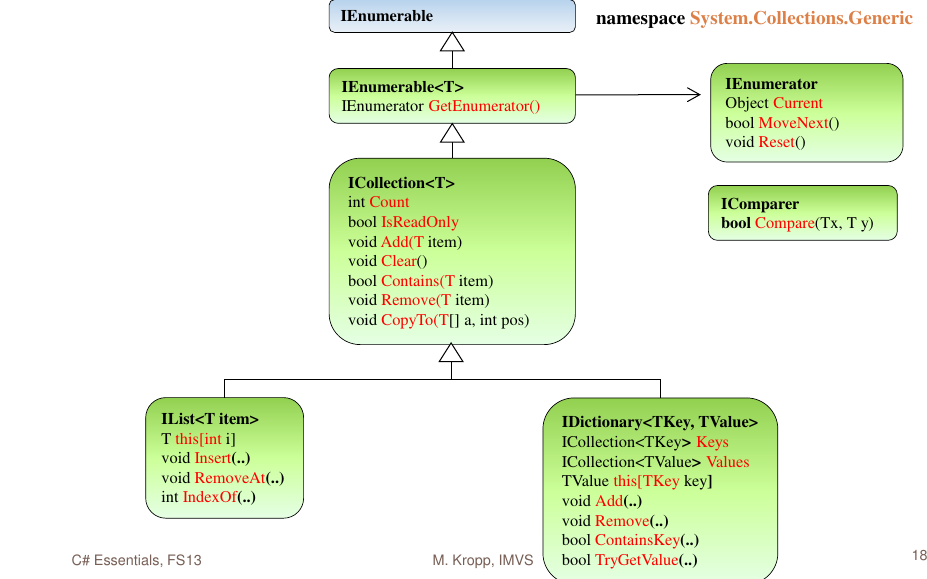
\includegraphics[scale=0.5]{./collections2.png}
 % collections1.png: 852x538 pixel, 96dpi, 22.54x14.23 cm, bb=0 0 639 403
 \caption{Generic Collections}
\end{figure}

\subsection{Switch Anweisungen}
\begin{lstlisting}[caption=Switch Anweisung]
 switch (country) {
  case "England": case "USA":
    language = "English";
  break;
  case "Germany": case "Austria": case "Switzerland":
    language = "German";
  break;
  case null:
    Console.WriteLine("no country specified");
  break;
  default:
  Console.WriteLine("don't know the language of " + country);
  break;
}

//Bemerkung keine Fall through - alles muss mit break return goto oder throw terminiert werden.
// Typen : int,char,enum,oder string, oder null
\end{lstlisting}

\subsection{Control Statements}

\begin{lstlisting}[caption=foreach Beispiel]
 foreach (char c in "beers"){
  Console.WriteLine(c);
 }
\end{lstlisting}

\begin{description}
 \item [break] Endet Schliefe oder switch.
 \item [continue] Macht nächste Iteration der Schliefe.
 \item [goto] ist des Teufels
\end{description}

\subsection{Arrays}
\begin{figure}[h]
 \centering
 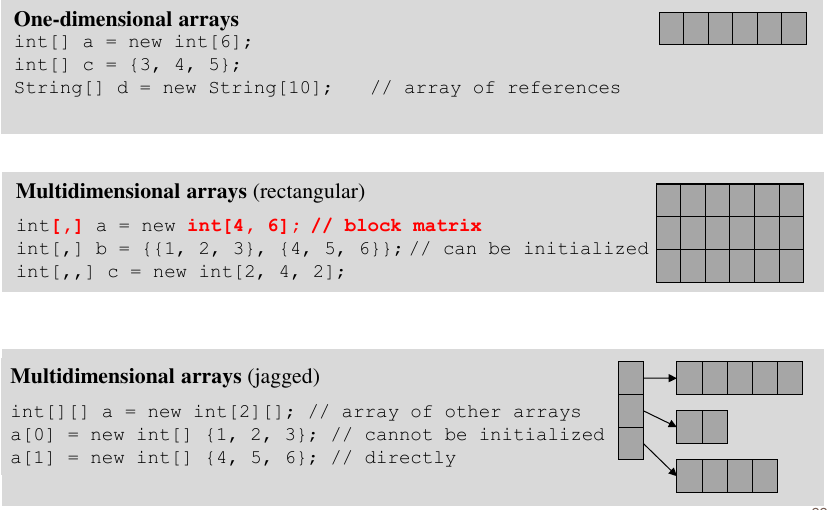
\includegraphics[scale=0.5]{./arrays.png}
 % arrays.png: 835x510 pixel, 96dpi, 22.09x13.49 cm, bb=0 0 626 382
 \caption{Arrays}
\end{figure}

\subsection{Variablen - Stack + Heap}

\begin{description}
 \item [Stack + Heap]
 \subitem Valuetypen sind immer auf dem Stack.
 \subitem Referenztypen sind auf dem Heap (Objekten new operator usw.) Garbage collection hier.
 \item [Definite Assignment] Definitive Zuweisung - Unmöglich uninitializierte Hauptspeicher zuzugreifen.
 \subitem Lokale Variablen : 1) Init 2) Zugriff.
 \subitem Felder + Arrays = Automatische Init.
\end{description}

\subsubsection{Dynamische Variablen}
\begin{lstlisting}[caption=Dynamische Variablen]
 var x = 5; // is equivalent to int x = 5; implicit type assignment, compile time checking
dynamic d = 5; // really dynamic, runtime checking
d‏=‏“hello”;

\end{lstlisting}

\subsection{Parameter}
\begin{lstlisting}[caption=Parameter Beispiel]
 //Modifiers
 void Parameters(int i, ref int ref_i, out int out_i)
 //Variable Anzahl parameter mussen letzte Paramter sein
void Parameters(int i, params int[] ints)
\end{lstlisting}

\subsection{Partial Classes}
Eine Klasse über mehrere Dateien.
VS.Net Trennung - Hand von generierte Code. Nicht nötig.

\subsection{Typechecking und Casting}
\begin{figure}[h]
 \centering
 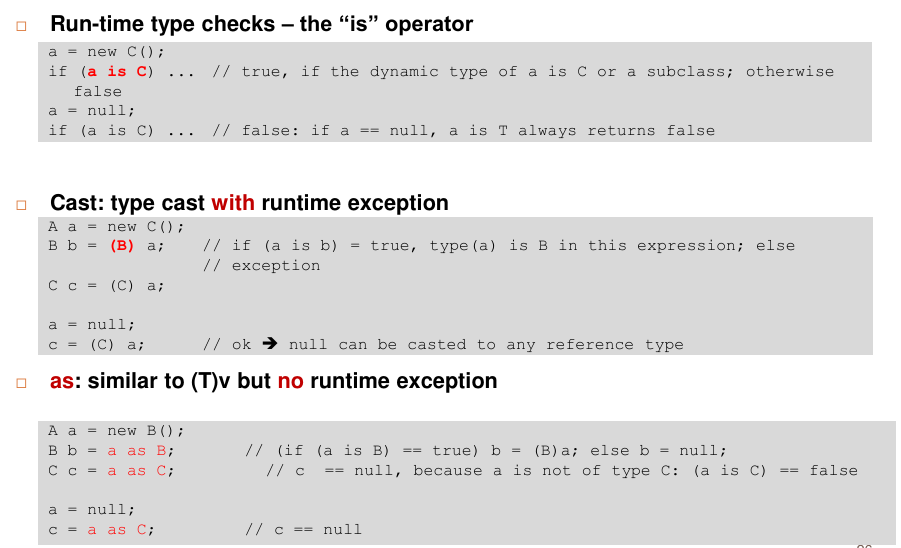
\includegraphics[scale=0.5]{./casting.png}
 % casting.png: 901x548 pixel, 96dpi, 23.84x14.50 cm, bb=0 0 676 411
 \caption{Typcheck + Casting}
\end{figure}

\subsection{Vererbung}

\begin{lstlisting}[caption=Vererbungsbeispiel]
 class B : A {
 // subclass (inherits from A, extends A)
int b;
public B() {...}
public void G() {...}
}
\end{lstlisting}
\begin{itemize}
 \item Konstruktoren nicht vererbt.
 \item Vererbte methoden können überschrieben werden.
 \item \textbf{Single Inheritance} nur von einer einzigen Klasse ableitbar.
 \item Klasse kann nur von einer Klasse vererben.
 \item Klasse ohne Vererbung vererbt automatisch von \texttt{Object}
\end{itemize}

\subsection{Override /Methodenüberschreibung}
\begin{lstlisting}[caption=Override Beispiel]
 class A {
    public void F() {...} // cannot be overridden
    public virtual void G() {...} // can be overridden in a subclass
}

class B : A {
// warning: hides inherited F(), default is new
  public void F() {...}
// warning: hides inherited G(), default is new
  public void G() {...}
  public override void G() { // ok: overrides inherited G
  ...
  }
}

\end{lstlisting}

\begin{itemize}
 \item Methodensignaturen müssen identisch sein.
 \item Properties und Indexers auch überschreibbar (virtual/override)
 \item \textbf{Statische  Methoden können nicht überschreiben werden}
\end{itemize}

\subsection{Methoden verstecken}
New Keyword muss benutzt werden.
\begin{lstlisting}[caption=Versteckung Beispiel]
class A {
public int x;
public void F() {...}
public virtual void G(){...}
}

class B : A
 {
public
 new int x;
public
 new void F() {...}
public
 new void G() {...}
}


B b = new B();
b.x = ...;
b.F(); ... b.G();
// accesses B.x
// calls B.F and B.G
((A)b).x = ...;
 // accesses A.x!
((A)b).F(); ... ((A)b).G();
 // calls A.F and A.G!

\end{lstlisting}

\subsubsection{Base Konstruktor aufrufen}
\begin{lstlisting}[caption=Basiskonstruktor implizit aufrufen]
 class A {
...
}
class B : A {
 public B(int x) {...}
 }
 
 // A() dann B(int x)
 class A {
public A() {...}
}
 class B : A {
  public B(int x) {...}
  }
 //das gleiche
 
 class A {
public A(int x) {...}
}
 class B : A {
 public B(int x) {...}
 }
 B b = new B(3);

 //Error : A hat kein Defaultkonstruktor mehr.
 
\end{lstlisting}

\begin{lstlisting}[caption=Basiskonstruktor explizit aufrufen]
 class A {
public A(int x) {...}
}
class B : A {
public B(int x)
: base(x) {...}
}
// A(int x) dann B(int x)
\end{lstlisting}

\subsection{Generics}
\begin{lstlisting}[caption=Generics Beispiel]
class Buffer <Element, Priority> {
private Element[] data;
private Priority[] prio;
public void Put(Element x, Priority prio) {...}
public void Get(out Element x, out Priority prio) {...}
}

Buffer<int, int> a = new Buffer<int, int>();
a.Put(100, 0);
int elem, prio;
a.Get(out elem, out prio);
Buffer<Rectangle, double> b = new Buffer<Rectangle, double>();
b.Put(new Rectangle(), 0.5);
Rectangle r; double prio;
b.Get(out r, out prio);

//GENERICS MIT CONSTRAINTS

class OrderedBuffer <Element, Priority> where Priority: IComparable {
Element[] data;
Priority[] prio;
int lastElem;
 interface or base class
...
// sorts x according to its priority into buffer
public void Put(Element x, Priority p) {
int i = lastElement;
while (i >= 0 && p.CompareTo(prio[i]) > 0) {
data[i+1] = data[i]; prio[i+1] = prio[i]; i--;}
data[i+1] = x; prio[i+1] = p;
}
}

OrderedBuffer<int, int> a = new OrderedBuffer<int, int>();
a.Put(100, 3);

//Ordered buffer implementiert IComparable
\end{lstlisting}

\subsubsection{Generics und Vererbung}
\begin{lstlisting}[caption=Generics und Vererbung]
 class Buffer <Element>: List<Element> {
...
public void Put(Element x) {
this.Add(x); // Add is inherited from List
}

}

// from a non-generic class
class T<X>: B {...}
//T from an concrete generic class
 class T<X>: B<int> {...}
 //from a generic class
//with the same placeholder
class T<X>: B<X> {...}

//CONSTRAINTS

public class BaseClass<T> where T : ISomeInterface
{...}
 public class SubClass<T> : BaseClass<T> where T: ISomeInterface
{...}


\end{lstlisting}

\subsubsection{Generic Methods}
\begin{lstlisting}[caption=Generische Methoden]
 static void Sort<T> (T[] a) where T: IComparable {
    for (int i = 0; i < a.Length-1; i++) {
      for (int j = i+1; j < a.Length; j++) {
	if (a[j].CompareTo(a[i]) < 0) {
	  T x = a[i]; a[i] = a[j]; a[j] = x; }
	}
    }
}

int[] a = {3, 7, 2, 5, 3};
...
Sort<int>(a);
//Typ inferenz hier, man muss nicht <int> angeben.
\end{lstlisting}

\subsection{FILE/IO}
\begin{figure}[h]
 \centering
 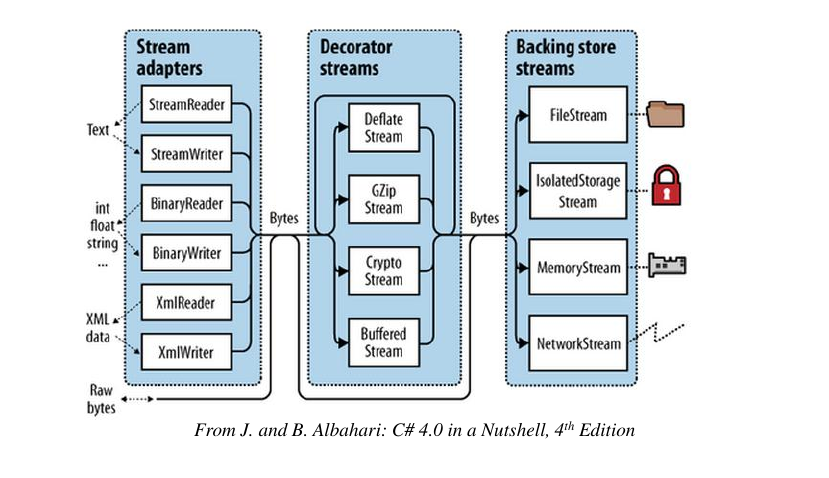
\includegraphics[scale=0.5]{./ioarch.png}
 % ioarch.png: 829x478 pixel, 96dpi, 21.93x12.65 cm, bb=0 0 622 358
 \caption{IO Architektur}
\end{figure}

\begin{lstlisting}[caption=Stream Beispiele]
 Stream stream = new FileStream("test.txt", FileMode.Create);
Console.WriteLine(stream.CanRead); // true
Console.WriteLine(stream.CanWrite); // true
Console.WriteLine(stream.CanSeek); // true
stream.WriteByte(201);
stream.WriteByte(210);
stream.Position = 0;
Console.WriteLine(stream.ReadByte());
stream.Close();

string filename = "Text.txt";
TextWriter writer= new StreamWriter(filename);
writer.WriteLine("First line.");
writer.WriteLine("Last line.");
writer.Close();
TextReader reader = new StreamReader(filename);
Console.WriteLine(reader.ReadLine());
Console.WriteLine(reader.ReadLine());
reader.Close()


\end{lstlisting}

\section{Delegates}

\subsection{Java vs c\# Delegate}
\begin{lstlisting}[basicstyle=\footnotesize\ttfamily]
 class MyComparator implements Comparator<Integer> {
@Override
public int compare(Integer o1, Integer o2) {
return (o1>o2 ? -1 : (o1==o2 ? 0 : 1));
}
...

Collections.sort ( list , new MyComparator()) ;

c#
// public delegate int Comparison<in T>(T x, T y);
Comparison<int> myComparer = delegate(int i1, int i2)
{
return i1.CompareTo(i2);
};
list.Sort(myComparer);

 The Sort-Method Interface
List<T>.Sort(Comparison<T> comparison);
In Fact: You can use any method following the
required delegate interface

\end{lstlisting}

\subsection{Nutzung von Delegates}
Ein Delegate ist ein Referenztyp dass einen Methodensignatur definiert.
\begin{lstlisting}[caption=Delegate Intro]
//muster
delegate returnType DelegateName([DelArguments]);

//beispiel
// method signature with keyword delegate
delegate void Notifier(string sender);
Notifier greetings;
void SayHello(string sender) { // just provide same interface
Console.WriteLine("Hello from " + sender);
}

greetings = new Notifier(SayHello) // full version, or
greetings = SayHello; // simplified assignment: delegate type
// is inferred from the type of the
// left-hand side

greetings("John");
 // invokes SayHello("John")
 
 //invoke another method
 
 void SayGoodBye(string sender) { // just another method
Console.WriteLine("Good bye " + sender);
}
greetings = SayGoodBye;
 // assign the method
greetings("John"); // SayGoodBye("John") => "Good bye John"


\end{lstlisting}
\textbf{Bemerkungen}
\begin{itemize}
 \item Delegate Variable kann null sein.
 \item Exception bei aufruf von diese Nullvariable.
 \item Delegateobjekten sind Objekten der ersten Klasse : können als Parameter benutzt weden oder in Datenstruktur gespeichert werden.
\end{itemize}


\subsection{Delegate Characteristics}

\begin{itemize}
 \item Delegates sind objektorientierte , typsichere und sicher, Funktionszeiger. 
  \subitem Delegateinstanz beinhaltet mehere Methoden die statisch oder nicht statisch sein können.
  \item Delegates erlauben dass man Methoden als Parameter übergeben kann.
  \item Benutzt um ``callback'' Methoden zu fefinieren.
  \item Chaining : Mehrere Methoden können bei einem Event aufgerufen werden.
  \item Grundlage für net Eventbehandelung.
  \item Delegate speichert Methodenname aber keine Parameter.
  \item Methoden müssen nicht abstrakt sein, aber können virtual ,override oder new Methoden sein.
  \item Delegate Typsignatur muss gleich Methodensignatur sein.
  \item Delegate kann mehrere Methoden gleichzeitig beinhalten.\textbf(Multicast Delegate)
  \subitem Falls es eine Funktion ist, wird der Wert des letzten Aufrufs züruckgegeben.
  \subitem Falls es ein \texttt{out} Parameter hat, wird der Parameter des letzten Aufrufs züruckgegeben.
  \subitem Ref Parameter sind durch alle Methoden weitergeleitet.
  
\end{itemize}

\subsection{Observer Pattern}
Stock watcher Beispiel :
\begin{figure}[h]
 \centering
 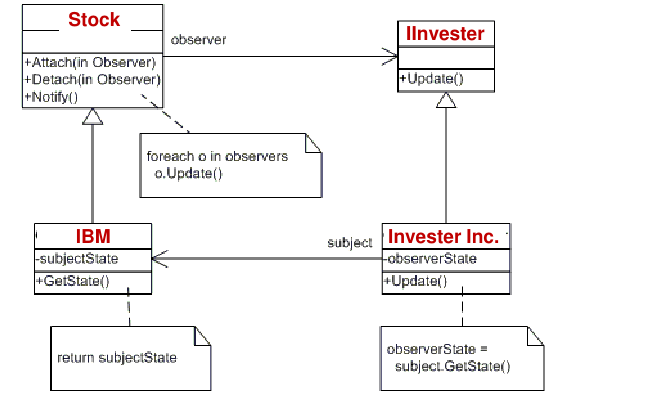
\includegraphics[scale=0.5]{./swatcher1.png}
 % swatcher1.png: 658x419 pixel, 96dpi, 17.41x11.08 cm, bb=0 0 493 314
 \caption{stock watcher java}
\end{figure}
\begin{figure}[h]
 \centering
 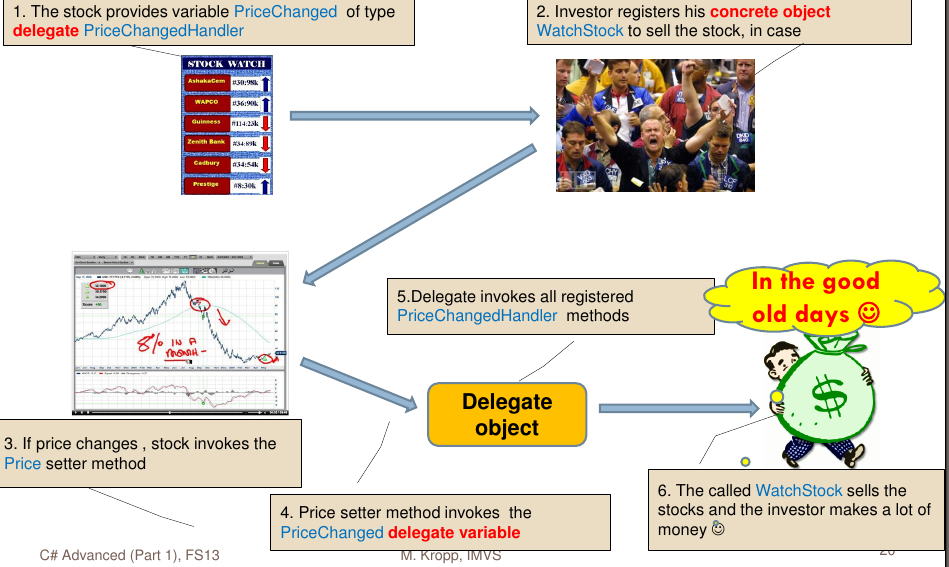
\includegraphics[scale=0.5]{./swatcher2.png}
 % swatcher1.png: 658x419 pixel, 96dpi, 17.41x11.08 cm, bb=0 0 493 314
 \caption{stock watcher c\#}
\end{figure}
\pagebreak
\begin{lstlisting}[caption=KeyHandler Beispiel]
public delegate void KeyEventHandler (object sender, KeyEventArgs e);
public class KeyEventArgs : EventArgs {
public virtual bool Alt { get {...} }
 // true if Alt key was pressed
public virtual bool Shift { get {...} } // true if Shift key was pressed
public
 bool Control { get {...} } // true if Ctrl key was pressed
public
 bool Handled { get{...} set {...} } // indicates if event
// was already handled
public
 int
 KeyValue { get {...} } // the typed keyboard code
... }
class MyKeyEventSource {
public event KeyEventHandler KeyDown;
public KeyPressed() {
KeyDown(this, new KeyEventArgs(...));
}
}
class MyKeyListener {
public MyKeyListener(...) { keySource.KeyDown += HandleKey;}
void HandleKey (object sender, KeyEventArgs e) {...}
}

 
\end{lstlisting}

\subsection{Predicate Delegates}


Delegate der einen Boolean züruckgibt. \\
\begin{lstlisting}[caption=Predicate Beispiel]
 class List<T > {
...
List<T> FindAll(Predicate<T> match);
T Find(Predicate<T> match);
int FindIndex(Predicate<T> match);
...}

public delegate bool Predicate<T> ( T obj )


bool ProductGT10(Point p)
{
if (p.X * p.Y > 100000){
return true;
}
return false;
}


//Annonymous

List<Point> FindWithAnonymousDelegate(List<Point> list)
{
return list.FindAll(delegate(Point p)
{ // here starts the anonymous method
if (p.X * p.Y > 100) { return true; }
return false;
});
}

\end{lstlisting}

\subsection{Func + Action Delegates}
\begin{lstlisting}[caption=Func Delegate]
 delegate TResult Func<out TResult> ();
delegate TResult Func<in T, out TResult> (T arg);
delegate TResult Func<in T1, in T2, out TResult> (T1 arg1, T2 arg2);

public static void FuncDelegateSample() {
Func<string, string> convertMethod = UppercaseString;
Console.WriteLine(convertMethod("Dakota"));
}
private static string UppercaseString(string inputString) {
return inputString.ToUpper();
}


\end{lstlisting}
\begin{lstlisting}[caption=Action Delegate]
 delegate void Action ();
delegate void Action<in T> (T arg);
delegate void Action<in T1, in T2> (T1 arg1, T2 arg2);

private static void ActionDelegateSample()
{
Action<string> act = ShowMessage;
act("C# language");
}
private static void ShowMessage(string message)
{
Console.WriteLine(message);
}

\end{lstlisting}

\subsection{Exceptions}
\begin{lstlisting}[caption=Exception Beispiel]
 FileStream s = null;
try {
s = new FileStream(curName, FileMode.Open);
...
} catch (FileNotFoundException e) {
Console.WriteLine("file {0} not found", e.FileName);
} catch (IOException) {
Console.WriteLine("some IO exception occurred");
} catch {
Console.WriteLine("some unknown error occurred");
} finally {
if (s != null) s.Close();
}

\end{lstlisting}

\subsubsection{Exception Characteristics}
\begin{description}
 \item Catch Klausel in sequenziellen Reihenfolge abgearbeitet.
 \item Finally wird immer ausgeführt.
 \item Exception Parametername kann weggelassen werden im Catchklausel.
 \item Exceptions immer von \texttt{System.Exception} abgeleitet.
 \item[Catchklauselbehandelung] Kette wird Ruckwärts travasiert bis Methode mit passende Catchklausel gefunden ist. Falls nicht dann Stack trace.
 \item [Fangen von Exceptions] Müssen nicht sein. Keine Unterschiede zwischen Checked und Unchecked Exceptions.
\end{description}

\section{Operator Overloading}
\begin{lstlisting}[caption=Operator Overloading Beispiel]
 public struct Rational {
...
public static Rational operator+ (Rational lhs, Rational rhs)
{
// here comes the implementation
return new Rational(...);
}
}

Rational r3 = r1 + r2;
r3 += r2; // !!! Provided for FREE
public override bool Equals(object o)

public static bool operator== (Rational lhs, Rational rhs)
public static bool operator!= (Rational lhs, Rational rhs)
if ( r1.Equals(r2) ) { ... }
 if ( !r1.Equals(r2)) { ... }
if ( r1 == r2 ) { ... }
 if ( r1 != r2 )
 { ... }

 public struct Rational {
...
public static implicit operator Rational(int i)
{
return new Rational(i,1);
}
}
 From int to Rational
Rational r = 2;

public struct Rational {
...
public static explicit operator double(Rational r)
{
return (double) r.Numerator / r.Denominator;
}
}

 From Rational to double
Rational r = new Rational(2,3);
double d = (double) r;

\end{lstlisting}

\section{Extension Methods}
\begin{lstlisting}[caption=Extension Methods Beispiel]
 public static String Concat(this String[] arr, String sep) {
StringBuilder sb = new StringBuilder();
sb.Append(arr[0]);
for (int i=1; i<arr.Length; i++)
sb.Append(sep).Append(arr[i]);
}
returnsb.ToString();
 Just call the new method, as it would be a regular string method
String[] stringArray = { "www", „fhnw", „ch" };
Console.WriteLine(stringArray.Concat("."));


namespace MyExtensions {
public static class MyExtensionsClass {
public static void MyMethod(this My my) {...}
}
}
 Use namespaces and using to control scope
namespace N1 {
using MyExtensions;
// My.MyMethod usable here
}
namespace N2 {
// My.MyMethod not usable here
}
\end{lstlisting}

\subsection{Objekt erweitern (vorsicht)}
\begin{lstlisting}[caption=Objekt Extension Method]
 public static class ObjectExtensions {
public static String ToString(this Object receiver,
params Object[] args) {
return "ToString, idiot!"; } }

\end{lstlisting}
\begin{itemize}
 \item Vorsicht mit Methoden im Scope von Ausländischer Namespace.
 \item Vorsicht welche Klassen haben Erweiterungen.
 \item Diese Methode kann auf irgendwelche Objekt benutzt werden.
 
\end{itemize}

\section{Yield}
\begin{lstlisting}[caption=yield Beispiel]
 public static IEnumerable<int> DoTest(int num) {
for (int i = 0; i < num; i++) {
yield return i;
}
yield break;
}
static void Main(string[] args) {
foreach (int num in DoTest(8)) {
Console.WriteLine(num);
}
}

public
  yield static return IEnumerable<int> and yield To(this break
 int first, int last)
{
 Must for (var return i = IEnumerator first; i <= last; or i++)
 IEnumerable
{
yield return i;
}
}
foreach (int i in 3.To(10))
{
j = i*i;
}


\end{lstlisting}

Yield packt allles automatisch in return typ ein im Hintergrund.

\subsection{Yield Einshränkungen}

\begin{enumerate}
 \item Gibt immer IEnumerator oder IEnumerable züruck.
 \item Nur innerhalb Iterator Block.
 \item Unsafe Blocks nicht erlaubt.
 \item Parameter fpr Methode, Operator oder Accessor können nicht \texttt{ref} oder \texttt{out} sein.
 \item Nicht in annonymen Methoden erlaubt.
\end{enumerate}

\section{Sicher und Unsicheren code}
Spezieller Modus : unsafe. Erlaubt pointers. Es ist aber nicht verifizirtbar und admin Rechte sind nötig. PInkvoke mechanismus?
GC + Pinning.\\
Man kann : \\
\begin{enumerate}
 \item Pointers deklarieren und benutzen.
 \item Konvertierungen zwischen Pointers und Basistypen machen.
 \item Nehme Adressen von variablen und weitere c++ sachen.
\end{enumerate}

\begin{lstlisting}[caption=Unsafe Code Example]
 class TestPointer
   {
      public unsafe static void Main()
      {
         int[]  list = {10, 100, 200};
         fixed(int *ptr = list)

         /* let us have array address in pointer */
         for ( int i = 0; i < 3; i++)
         {
            Console.WriteLine("Address of list[{0}]={1}",i,(int)(ptr + i));
            Console.WriteLine("Value of list[{0}]={1}", i, *(ptr + i));
         }
         Console.ReadKey();
      }
   }
}
\end{lstlisting}

\subsection{Pointer Operations}
\begin{tabular}{l | l}
Pointer Element access & \begin{lstlisting}
                         char *p 
                         \end{lstlisting} \\
Adress-of Operator & \begin{lstlisting}
                      unsafe int i; &l
                     \end{lstlisting}\\
Pointer Arithmetik & \begin{lstlisting}
                      char *p; p++;
                     \end{lstlisting}\\
sizeof Operator & \begin{lstlisting}
                   sizeof(byte)
                  \end{lstlisting}\\
stackalloc & \begin{lstlisting}
              stackalloc int[10]
             \end{lstlisting}\\
Fixed statement & fixed \\ 
\end{tabular}

\subsection{Pinning Objects}
\begin{lstlisting}[caption=Pinning Objects]
 public void FixVar2()
{
string strName = "Fixing Variables";
unsafe
{
fixed( char* pStr = strName )
{
for ( int i = 0; pStr[i] != '\0'; i++)
System.Diagnostics.Trace.Write( pStr[i] );
}
}
}

//The fixed statement prevents relocation of a variable by the garbage collector in
//unsafe contexts only.

\end{lstlisting}

\section{Reflection}
\subsection{Reflection Grundkonzepte}
\begin{description}
 \item [Metadata] \hfill \\
 \subitem Einzige Ort für Typ Info und Code
 \subitem Code ist innerhalb Typinfo beinhaltet.
 \subitem Jede Objekt kann für seinen Typ abgefragt werden.
 \subitem Metadata von Typen kann mit Reflection entdeckt werden.
 \item [Dynamic Type System] \hfill \\
 \item Sehr dynamisch und Spracheunanbhängig.
 \item Typen können erweitert werden und gebaut werden zur Laufzeit.
 \item ``On the fly'' erzeugung von Assemblies (dlls).
\end{description}

\subsection{Type Info zur Laufzeit}
\begin{figure}[h]
 \centering
 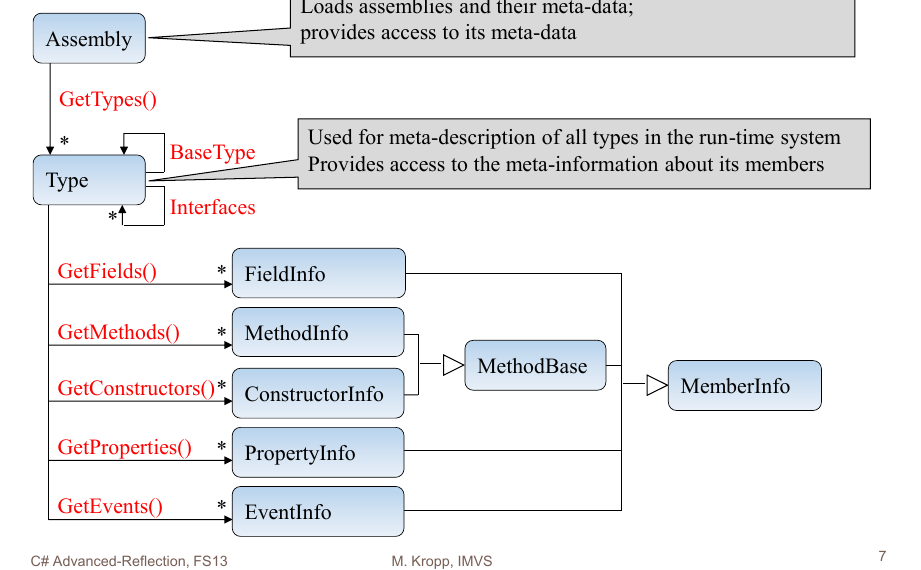
\includegraphics[scale=0.5]{./reflection1.png}
 % reflection1.png: 921x570 pixel, 96dpi, 24.37x15.08 cm, bb=0 0 691 427
 \caption{Typ Info zur Laufzeit}
\end{figure}

\subsection{Laden von Assemblies}
\begin{lstlisting}[caption=Laden von Assemblies]
 Assembly a = Assembly.LoadFrom("HelloWorld.exe");
Type[] types = a.GetTypes();
foreach (Type t in types)
Console.WriteLine(t.FullName);

Type hw = a.GetType("Hello.HelloWorld");
MethodInfo[] methods = hw.GetMethods();
foreach (MethodInfo m in methods)
Console.WriteLine(m.Name);

\end{lstlisting}
\begin{description}
 \item [System.Type] \hfill \\
 \subitem Zugriff auf Metadata für alle net Types.
 \subitem Rückgabewert von Object . getType()
 \subitem zugriff auf Methoden Konstruktoren , Parametern, Feldern, Properties,Argumente,Atributen,Events,Delegates,Namespaces.
\end{description}

\subsection{Innerhalb Typinfo}
\begin{description}
 \item [Members Entdecken]
 \subitem [MemberInfo] \texttt{GetMembers(),FindMembers()}
 \item [Felder + Properties Entdecken]
 \subitem [MemberInfo] \texttt{GetFields(),PropertyInfo : GetProperties()}
 \item [Konstruktoren Entdecken]
 \subitem \texttt{GetConstructors(),GetMethods(),GetEvents()}
\end{description}

\subsubsection{MemberInfo}
\begin{figure}[h]
 \centering
 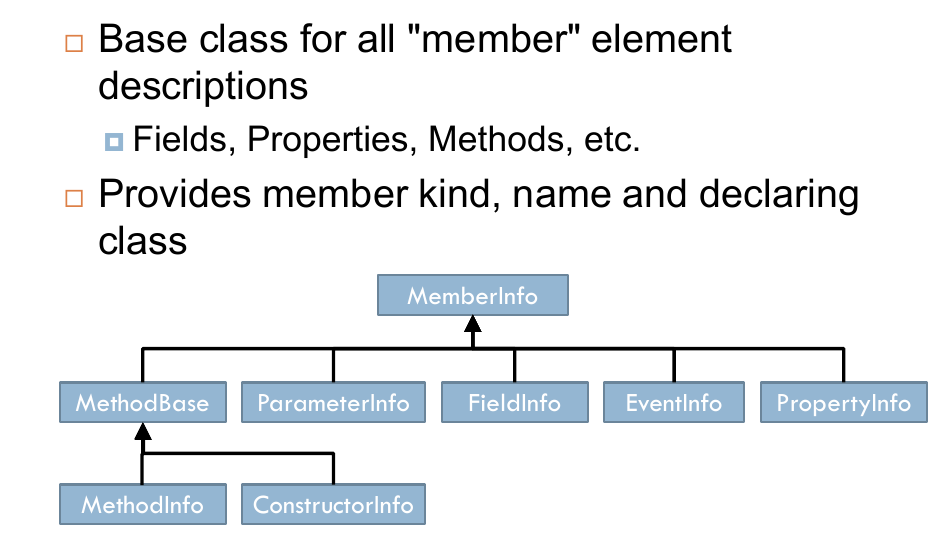
\includegraphics[scale=0.5]{./reflection2.png}
 % reflection2.png: 939x544 pixel, 96dpi, 24.84x14.39 cm, bb=0 0 704 408
 \caption{Memberinfo Diagramm}
\end{figure}

\subsection{Bigger Picture}
\begin{figure}[h]
 \centering
 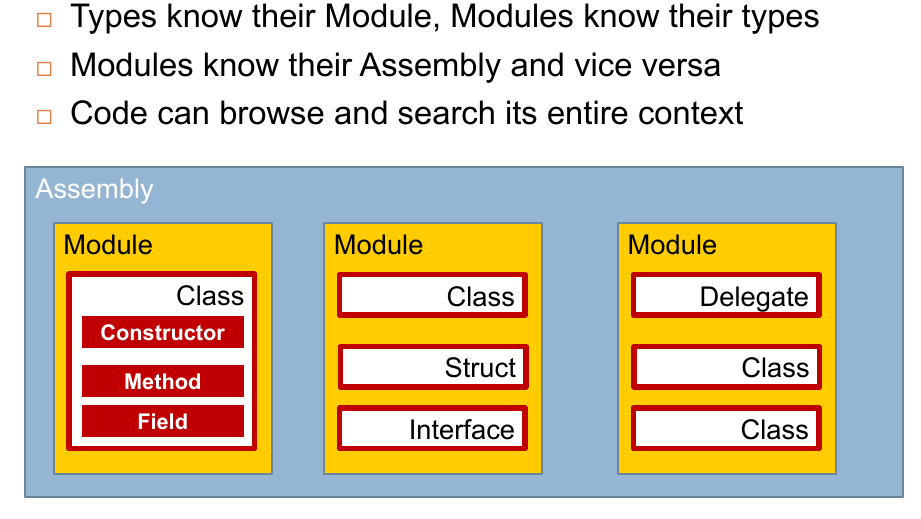
\includegraphics[scale=0.5]{./reflection3.png}
 % reflection2.png: 939x544 pixel, 96dpi, 24.84x14.39 cm, bb=0 0 704 408
 \caption{Macht von Reflexion}
\end{figure}

\section{Attributes}
\begin{itemize}
 \item Benutzerdefinierte MetaInfo über Programmelemente.
 \item Kann an alles geklebt werden.
 \item Kann zur Laufzeit abgefragt werden
 \item Erweitert vorherdefinierte Attributen wie public sealed oder abstract.
 \item Benutzt von CLR Servixes (serialization , COM usw)
 
\end{itemize}

\subsection{Benutzer definierte Attributen}
\begin{lstlisting}[caption=Benutzerdefinierte Attributen]
 /// causes compiler to bring message, that a class C is
/// obsolete
public class ObsoleteAttribute : Attribute {
public string Message { get {...} }
public bool IsError { get {...} set {...} }
public ObsoleteAttribute() {...}
public ObsoleteAttribute(string msg) {...}
public ObsoleteAttribute(string msg, bool error) {...}
}

//Positional Parameter : of attr constructor

[Obsolete(“Message Use class C1 instead", true)]
public class C {.. }

//Name Parameter : public property of attr class

 [Obsolete(IsError=true, Message=“Use class C1 instead")]
public class C {.. }
 
 //Mixed
[Obsolete(“Use class C1 instead“, IsError=true)]
public class C {.. }


\end{lstlisting}
\begin{lstlisting}[caption=Querying Attributes]
 class CommentAttribute : Attribute {
string text, author;
public string Text { get {return text;} }
public string Author { get {return author;} set {author = value;} }
public Comment (string text) { this.text = text; author ="HM"; }
}
[Comment("This is a demo class for Attributes", Author="XX")]
class C { ... }
class Test {
 search should
static void Main() {
 also be continued
Type t = typeof(C);
 in subclasses
object[] a = t.GetCustomAttributes(typeof(Comment), true);
Comment ca = (Comment)a[0];
Console.WriteLine(ca.Text + ", " + ca.Author);
}
}

\end{lstlisting}

\subsection{AttributeUsage}
\begin{lstlisting}[basicstyle=\footnotesize\ttfamily]
 
 Describes how user-defined attributes are to be used
public class AttributeUsageAttribute : Attribute {
public AttributeUsageAttribute (AttributeTargets validOn) {...}
public bool AllowMultiple { get; set; }
 // default: false
public bool Inherited { get; set; }
 // default: true
public AttributeTargets ValidOn { get; set; } // default: All
public virtual Object TypeId { get;}
}
validOn	to which program elements is the attribute applicable?
AllowMultiple	can it be applied to the same program element multiple times?
Inherited	is it inherited by subclasses?
TypeID	when implemented, gets unique identifier for derived attribute classes


Usage
[AttributeUsage(AttributeTargets.Class |
AttributeTargets.Interface, AllowMultiple=false)]
public class MyAttribute : Attribute {...}

\end{lstlisting}

\section{LINQ + Lambda}
\subsection{Lambda}
Drawback of annonymous methods :
\begin{itemize}
 \item Mthod must be implemented
 \item Annonymous methods are hard to read.
 \item Resricted usage
\end{itemize}


\begin{lstlisting}[caption=some basic lambda examples]

(parameters) => expression-or-statement-block


 List<Point> list = list.FindAll((p) =>
{
return (p.X * p.Y > 100000);
});

delegate int Transformer(int i);
We could assign and invoke the following
ambda expression
Transformer square = x => x*x; // Lambda expression

x => { return x * x; };

 Lambda’s are mostly used with FunAction delegate
Func <int, int> sqr = p => p * p;
Action showValue = i => Console.WriteLine(i);


\end{lstlisting}

The compiler converts these expressions into annonymous delegate methods or an expression tree.

\begin{lstlisting}[caption=lambdas and functions]
 Func <string, string, int> totalLength =
(s1, s2) => s1.Lenght + s2.Length;
 //Explicitly specified parameter types
Func <int, int> sqr = (int p) => p * p;
 //Otherwise the compiler uses type inference to determinthat x is an int
Func <int, int> sqr = p => p * p;

\end{lstlisting}

\subsubsection{Lambda Execution Context}
\pic[Lambda Execution Context]{lambda1.png}
\pic{lambda2.png}

\subsection{LINQ}
\subsection{Advantages and bla bla}
\begin{itemize}
 \item Type Safe,
 \item SQL Similarities,
 \item Query Set and Transform Operations for .net-
 \item Works with all types of data (xml,objects,db)
 \item Integrated part of .net Languages , enables language-based querying.
 
\end{itemize}

\begin{lstlisting}[caption=basic LINQ Examples]
  //Given a collection
ames = new List<String> { “Tom", “Dick”, “Harry”,
“Mary", “Jay” }
 //Search all names in list containing “a”
ar results = from n in names
where n.Contains(“a")
select n;
// Sort list
ar results = from n in names
orderby n
select n;

\end{lstlisting}

\subsubsection{LINQ General Syntax}
\begin{itemize}
 \item Query begins with from caluse, and ends with select or group clause.
 \item Clause Examples : Where , Orderby join, let , from , into
\end{itemize}
\subsubsection{LINQ Key Features}
\begin{enumerate}
 \item Deferred Execution. Retrieve, specific value, Itwerate through a collection perform a specific operation.
 \item Compile time syntax and schema checking.
 \item LINQ is abstracted from underlying data. Consistent across various data sources.
\end{enumerate}

\subsubsection{Query Chaining}
\begin{lstlisting}
 var query = from name in names
where name.Contains „a“
orderby name.Length
select name.ToUpper();
//filter->sorter->projector
\end{lstlisting}

\subsubsection{Formulating LINQ Expressions}
\begin{description}
 \item [Method or Fluent Syntax] \begin{lstlisting}
                                  var usCustomers = names
				  .Where(n=>n.Contains(„a“));

                                 \end{lstlisting}
\item[Query Comprehension Syntax]\begin{lstlisting}
                                  var usCustomers = from name in names
				  where n.Contains(„a“)
				  select n;

                                 \end{lstlisting}
\item[Hybrid Syntax] \begin{lstlisting}
                      var results = (from c in Comedians
		      select c).Count();
                     \end{lstlisting}


\end{description}

\subsubsection{LINQ and objects}

If an object supports the IEnumerable interface it is compatible with LINQ to Objects provider.

\subsubsection{Local vs Interpreted Query}
\begin{description}
 \item [Local] IEnumerable + Delegates
		\begin{lstlisting}
		 public static IEnumerable<TSource> Where<TSource>(
this IEnumerable<TSource> source,
Func<TSource, bool> predicate)

		\end{lstlisting}
\item[Interpreted] Queryable + Expression Trees
		  \begin{lstlisting}
		   public static IQueryable<TSource> Where<TSource>(
this IQueryable<TSource> source,
Expression<Func<TSource, bool>> predicate)

		  \end{lstlisting}


\end{description}
\subsubsection{Feature Summary}
\pic{lambda3.png}

\section{Dynamic Programming}

\subsection{Dynamic vs Static Languages}
\begin{description}
 \item [Dynamic] \begin{enumerate}
                  \item Simple and succinct.
                  \item Implicit Typing
                  \item Meta programming
                  \item No compilation.
                  
                 \end{enumerate}
\item[Static] \begin{itemize}
               \item Robust
               \item Performing
               \item Intelligent tools,
               \item Scalable
              \end{itemize}


\end{description}

\subsection{Dynamic Language Architecture}
\pic{lambda4.png}

\subsection{DLR Concepts}
\begin{description}
 \item [Expression Trees] Represent language semantics; enables creation of
new dynamic languages. Includes control flow,
assignment, other language-modeling nodes.
\item[Call-Site Caching] Optimization for faster dyamic binding.
\item [Dynamic Object Interop]  Dynamic binding and dispatching objects and method
calls
\end{description}

\textbf{DLR runs on top of CLR as additional layer}


\subsection{Using Dynamic}
\begin{lstlisting}[caption=using dynamic]
//Static
ScriptObject calc = GetCalculator();
object res = calc.Invoke("Add", 10, 20);
int sum = Convert.ToInt32(res);
//Dynamic
dynamic calc = GetCalculator();
int sum = calc.Add(10, 20);
dynamic x = 1;
dynamic y = "Hello";
dynamic z = new List<int> { 1, 2, 3 };

\end{lstlisting}

Member selection deferred to runtime, dynamic substituted at runtime. Static type is ``dynamic``

\subsection{Implementing Dynamic}
\begin{lstlisting}[caption=dynamic object example]
 class Duck : DynamicObject{
public override bool TryInvokeMember(
InvokeMemberBinder binder, object[] args,
out object result)
 {
Console.WriteLine(binder.Name + " method was called");
}
}
return true;
static void Main(string[] args){
dynamic duck = new Duck();
duck.Quack();
duck.Waddle();
}

\end{lstlisting}

\subsubsection{API}

\begin{description}
 \item [Call Dynamic Methods] \begin{lstlisting}
                               public virtual bool TryInvokeMember(InvokeBinder
binder,Object[] args, out Object result)

                              \end{lstlisting}
\item[Get Properties] \begin{lstlisting}
                       public virtual bool TryGetMember(GetMemberBinder
binder,out Object result)

                      \end{lstlisting}
                      
\item[Set Properties] \begin{lstlisting}
                       public virtual bool TryInvokeMember(InvokeBinder
binder,Object[] args, out Object result)

                      \end{lstlisting}

\end{description}

\subsection{Dynamic Language Integration - Python}
\begin{lstlisting}
 static object Calculate(string expression)
{
ScriptEngine engine = Python.CreateEngine();
return engine.Execute(expression);
}
static void Main(string[] args)
{
dynamic result = Calculate("2 * 3");
Console.WriteLine("result: {0}", result);
}

\end{lstlisting}

\subsubsection{Data Passing}
\begin{description}
\item [in] ScriptScope.SetVariable.
\item [out] ScriptEngine.GetVariable.
\end{description}

\subsection{COM Interop}
\begin{lstlisting}[caption=COM Interop Example]
 using Word = Microsoft.Office.Interop.Word;
var word = new Word.Application();
word.Documents.Add();
Word._Document doc = word.ActiveDocument;
word.Selection.Text = "Demo test";
word.Selection.Paste();
doc.SaveAs(@"/test");
doc.Close();
word = null;

\end{lstlisting}

\textbf{Features}
\begin{itemize}
 \item Optional and Named Params.
 \item Indexed Properties
 \item Optional Ref modifiers.
 \item Interop Type Embedding.
\end{itemize}

\subsection{Native Code}
Can be done in one of two ways : Explicit P/Invoke (DLL Import) or Implicit P/Invoke (C++ Interop).\\

\begin{lstlisting}[caption=Explicit PInvoke example]
// Assume that we have the following Win32
function (in C)
int MessageBox (HWND hWnd, LPTSTR lpText, LPTSTR lpCaption, UINT
uType);
//We can invoke it from C#
using System;
System.Runtime.InteropServices;
class Test {
[DllImport("user32.dll")]
static extern int MessageBox(uint hWnd, string text, string
caption, uint type);
 // no body
static void Main() {
int res = MessageBox(0, "Isn't that cool?", "", 1);
Console.WriteLine("res = " + res);
}
}

\end{lstlisting}

\subsubsection{DLL Import Structure}
\pic[DLL Import Structure]{dllimport.png}

\subsubsection{Parameter Marschling}
\pic[Parameter Marschalling]{pm.png}

\subsubsection{Passing Structs}
\pic[Passing Structs]{pstructs1.png}
\pic{pstructs2.png}
\pic{pstructs3.png}

\subsection{Implicit P Invoke C++}

Problems : Custom types Byte alignment  Memory Management Pointers Passing managed allocated memory.
\begin{lstlisting}[caption=Implicit PInvoke]
 // vcmcppv2_impl_dllimp.cpp
// compile with: /clr:pure user32.lib
using namespace System::Runtime::InteropServices;
// Implicit DLLImport specifying calling convention
extern "C" int __stdcall MessageBeep(int);

\end{lstlisting}

\section{Diagnostics and Garbage Collection}

\subsection{General}
\begin{enumerate}
 \item Allocate the object and forget about it - Automatic Memory management.
 \item If the heap does not have enough space for the new object, garbage collection occurs.
 \item Always call Dispose() on any object you directly create if the objects supports IDisposable.

\end{enumerate}


\subsection{Object Creation}
\begin{lstlisting}
 Car c = new Car(“Viper”, 200, 100);
 IL
IL_000c: newobj instance void CilNew.Car::.ctor (string, int32, int32)

\end{lstlisting}

Tasks for CIL new object instruction are : Calculating total memory, examining the managed heap to ensure that there is enough room.
Return the referece to the caller, and then advance the ''next object pointer`` to point at the next available object on the heap.
\pic[Garbage Collection with managed Heap]{gc1.png}

\subsection{GC in .net}
\textbf{Tracing garbage collector}. Determines reachable objects and then discards all the unreachable ones. 
Does not interfere with object access, but is a thread that wakes up intermittently and calculates the object graph - reachability.

\subsubsection{Reachability}
\begin{description}
 \item [Reachable Objects] reachable from roots via references, otherwise garbage.
 \item [Roots] Distinguished set of objects always reachable. Examples are static and global variables, locals and arguments on the stack,CPU Registers. Otherwise known as \textbf{Strong references}
\end{description}

\textbf{Determining Reachability}
\pic{reachability.png}

\subsubsection{Cleaning up objects}
\begin{lstlisting}[caption=c\# finalise]
 protected override void Finalize()
{
try { /* code */ }
finally { base.Finalize(); }
}

\end{lstlisting}

\begin{itemize}
 \item Prior to an object being released its finalizer is called.
 \item Overriding finalise can perform any memory cleanup for the type.
 \item Finalise is called in the following cases \textbf{this call is non deterministic} : 
  \subitem natural garbage collection
  \subitem GC.collect method.
  \subitem Application Domain is being unloaded from memory.
  \subitem CLR being shutdown
\end{itemize}

\subsubsection{The collection process}
\pic[Garbage collection Process]{gcprocess.png}

\subsubsection{Finilisation guidelines}
\begin{enumerate}
 \item Override in case of unmanaged rescources (c++ pinvoke)
 \item Dont use unecessarily.
 \item make finalised objects as small as possible
 \item dont use referenced fields in finalised objects.
 \item dont access above field in finalised method.
\end{enumerate}

\subsection{Explicit Rescource Management}
Some objects require explicit tear down. IDisposable interface is made for this purpose. A programmer must exclusively call dispose method of object to perform cleanup.
Structures and classes support Idisposable, finalise is only overrideable on classes. Can also be used along with finalise.

\begin{lstlisting}[caption=Idisposable example]
 // Implementing IDisposable
public class MyResourceWrapper : IDisposable
{
// The object user should call this method
// when they finished with the object.
public void Dispose()
{
// Clean up unmanaged resources here.
// Dispose other contained disposable objects.
}
}

\end{lstlisting}

\subsubsection{Semantics}
\begin{enumerate}
 \item Disposed = beyond redemption. No reactivation, call on disposed object throws disposed exception.
 \item calls to dispose can be repeated
 \item A containing object should call dispose of all its children.
\end{enumerate}

\subsubsection{Dispose Pattern}
\begin{description}
 \item [Scope] Classes that are not sealed and require rescource cleanup.
 \item [Purpose]  The pattern has been designed to ensure reliable, predictable
cleanup, to prevent temporary resource leaks, and to provide
a standard, unambiguous pattern for disposable classes. It
also aids subclasses to correctly release base class
resources.

\end{description}

\begin{lstlisting}[caption=Dispose Pattern Implementation]
 // thread-safe wrapper of some unmanaged handle:
public sealed class OSHandle : IDisposable
{
private bool disposed;
public OSHandle(IntPtr h) { handle = h; disposed = 0; }
public void Dispose()
{
Dispose(true);
GC.SuppressFinalize(this);
}
~OSHandle() {
Dispose(false);
}

void Dispose(bool disposing)
{
if (!disposed){
}
// clean-up:
if (disposing) {
/* safe to access reference fields here */
}
disposed = true;
// dispose unmanaged resources here
}
base.Dispose(disposed);
}
\end{lstlisting}

\textbf{Using statements automatically call dispose on all objects within brackets of the statement, at the end.}

\subsubsection{Finalise vs Dispose}
\begin{description}
 \item [Finalise] Called by GC , not deterministic, fully auto, Used to free memory,
 \item [Dispose] Deterministic,explicit call,Free rescources - file locks etc.
\end{description}

\subsection{System.GC}
Interaction with garbage collector. Use when creating types that use unmanaged resource.

\subsection{GC Explained}
Divided into two Phases. Detection and reclamation. Detection is when objects are no longer used, reclamation is a release for memory use.
Each phase has various techniques and algorithms.

\textbf{Garbage collection steps}
\begin{enumerate}
 \item Detection : searches for managed objects that are referenced in managed code. (mark)
 \item Reclamation :  finalise unreachable objects. (sweep)
 \item Free unmarked objects and reclaim memory. (sweep)
\end{enumerate}
\pic[Garbage collector visualised]{gcvisual.png}

\section{Assembly and CIL}
\subsection{Role of Assemblies}
\begin{enumerate}
 \item Reuse of Code - smallest executable unit.
 \item Type boundry - types are usually unique.
 \item Versionable Units.
 \item Contain all type info - self describing.
 \item Cofngurable can be stored anywhere. 
 
\end{enumerate}
\pic[Assembly Content]{asmcontent.png}

\subsection{Tools}
\begin{description}
 \item [Compilers] csc.exe or vbc.exe.
 \item [IL assembler] ilasm.exe
 \item [IL dissasembler] ildasm.executable
 \item [Assembly Management] gacutil.executable
\end{description}

\subsection{Assembly Info}
Use assembly class. 
\begin{description}
 \item [Currently executing Assembly] GetExecutingAssembly()
 \item [Assembly of original entry method] GetEntryAssembly()
  \item [Assembly that called current function] GetCallingAssembly()
  \item [Assembly Attributes] assemblyinfo.cs or Reflection API \begin{lstlisting}
                                                                 GetCustomAttributes(typeof(AssemblyTitleAttribute), false);

                                                                \end{lstlisting}
  \item[Application Manifest] Assembly info for OS. Represented with external file or usually embedded.
  \item [Satellite Assemblies] external for resources.
  

\end{description}

\subsection{Managing Private Assemblies}
Usually stored in local bin dir, if not found gives exception. However can be stored anywhere provided it has been configured in App.Config.
\begin{lstlisting}
 <configuration>
<runtime>
<assemblyBinding xmlns="urn:schemas-microsoft-com:asm.v1">
<probing privatePath="MyLibraries"/>
</assemblyBinding>
</runtime>
</configuration>

\end{lstlisting}


\subsection{Make assembly available publicly}
\begin{verbatim}
 Location: C:\Windows\assembly (before .Net 4.0)
C:\Windows\Microsoft.NET\assembly (after .Net 4.0)

\end{verbatim}
\pic{gacinstall.png}
\begin{verbatim}
 The directory
C:\Windows\Microsoft.NET\assembly\GAC_MSIL\Accessibility\
2.0.0.0__b03f5f7f11d50a3a
\end{verbatim}

\subsubsection{Signing Assembly}
\pic{signgac.png}


\subsection{What is CIL}
Intermediate language between high level and machine code.
Lowest level before machine code/ similar to java byte code. Open standard , machine independant.
Advantages : Language interop - CIL code different languages, one program.
OS Portability.

\subsection{CIL}
\subsubsection{Hello world example}
\begin{lstlisting}
 .assembly extern mscorlib{...}
.assembly FirstGlance{...}
.module FirstGlance.dll
.class public auto ansi beforefieldinit HelloWorld
extends [mscorlib]System.Object
{
.method public hidebysig instance void
SayHello() cil managed
{
.maxstack 8
ldstr "Hello World"
call void [mscorlib]System.Console::WriteLine(string)
ret
}
}

\end{lstlisting}

\subsubsection{CIL Programming model}
All operations are stack not register based. Locals and incoming parameters live on stack.
Stack is of arbritrary size.

Names : everything has to be fully qualified.
\pic[IL Types]{cilnames.png}

\subsubsection{Execution State}
\pic[CIL Stack]{cilstack1.png}
\begin{description}
 \item [Activation Record] holds all per activation data of method. Used to implement method calls. 
 Contains : Arguments and local variables. Activation of method by a ''call`` instruction causes a new activation record to be created
 \item [Evaluation Stack] Operations performed on this stack. Stack used to store information just before the execution of a statement.It has 3 operations push,pop and perform
 \item [Logical Stack] Elements of stack are not of particular size. Depth = number of elements on stack.
 \item [Stack $\delta$] Instruction in IL to change depth of stack.
\end{description}
\pic[Stack Example operation]{stackexample.png}

\subsubsection{Base Instruction Set}
\begin{description}
 \item [Load and store Instructions] Push pop.
 \item [Operate Instructions] Arithmetic, logical, type conversion.
 \item [Branching and Jumping] Boolean vals, labels and jumps.
 
\end{description}

\pic[Loading and storing]{loadstore.png}
\pic[Loading and Storing 2]{loadstore2.png}
\pic[Operating Instructions]{opinst.png}

\subsubsection{Names and Directives in CIL}
\pic[Names in CIL]{cilnames.png}
\pic[Directives and Names]{cilnamedirective.png}.

\subsubsection{Value Classes /Structs}
\begin{lstlisting}
 
 //In c#:
public struct ValCls {public int I,j,k}

 //MSIL:
.class value public auto ansi sealed ValCls
extends [mscorlib]System.ValueTypes
{
.field public int32 I;
.field public int32 j;
.filed public int32 k;
}

\end{lstlisting}

\subsubsection{Class Declarations}
\begin{lstlisting}
 ClassDecl → .class ClassHeader”{”{MemberDecl}”}”
ClassHeader → {ClassAttr} ident [extends TypeRef]
[implements TypeRef {‘,’TypeRef}]
MemberDecl → <Member Declaration>
 class members: fields, methods, properties, events
.class public auto ansi Hello extends [mscorlib]System.Object
{
...
}

\end{lstlisting}

\textbf{Class Declaration Attribs}
\begin{tabular}{c c}
private & Default - Class and Members not visible outside assembly. Cannot be used with public. \\
public & Opposite of private. \\
abstract & Cannot be instantiated. \\
interface & interface definition. \\
sealed & cannot be extended. \\
ansi & ansi marschalling for strings - default \\
autochar & auto for character strings \\
unicode & unicode for character strings \\
auto & layout of class determined automatically \\
explicit & layout of class is explicit \\
sequential & sequential layout of class. \\
\end{tabular}

\subsubsection{Defining Methods}
\begin{lstlisting}
// MethodDeclaration
→ .method MethodHead ”{” {MethodBody} “}”
// MethodHead
→ { MethodAttr } [CallConv] TypeRef DottedName ‘(’ [Parameter
{‘,’ Parameter}] ‘)’ {ImplAttr}
.method public static void hello() cil managed
{
...
}

\end{lstlisting}

\subsubsection{Method bodies}
\pic[Method bodies]{methbod.png}

\section{Concurrency}

\subsection{Basic Concepts}
\begin{description}
 \item [Multitheading] Use of multiple Threads
 \item [Concurrency] Order in which multiple tasks execute is not determined.
 \item [Parallelism] True simultaneous multicore execution
\end{description}

Types of Asynchrony:
\begin{description}
 \item [IO Bound Async] Usually wait for response Goal is thread efficiency.
 \item [Computing Bound async] Responsive foreground behaviour during computing intensive tasks.
\end{description}

\subsection{.Net Async Concepts}

Async methods almost like sync code. Unifies comp, network and IO Async. Need for a more responsive UI.
\begin{description}
 \item [Threads] Low level. 
 \item [TPL] Parallel programing.
\end{description}

\subsection{Threads vs Tasks}
\begin{description}
 \item [Task] Future / Promise. Task<T> returns a T when task is done but not now.
 \item [Thread] One of many ways to fill promise above. \textit{Not every task needs a thread.} Sometimes the task only registers a callback, fully automated decision on whether thread is needed or not. 
 
\end{description}

\begin{lstlisting}[caption="task example"]
 
 // Step 1
 private Task<int> ComputeValueAsync(int start, int count)
{
var random = Task.Run(() =>
ComputeValue(start, count));
}
return random;

//Step 2 
int sum = await ComputeValueAsync(Start, Count);
Console.WriteLine("Result (synchronously) : {0}", sum);

//Step 3 
public async void DoLongRunningTask()
{
int sum = await ComputeValueAsync(Start, Count);
Console.WriteLine("Result (synchronously) : {0}",
sum);
}

\end{lstlisting}

\subsection{Task class API}
\begin{description}
 \item [Task.Run(somedelegate)] Static method starts a task, has many overloads.
 \item [Task.Wait] waits for task to complete. 
 \item[ Task<T> = Task.Run( someDelegate)] T is returning type of delegate.
 \item[TaskCompletionSource]  Another class to start and control task execution.
 \item Additionally there is cancellation and progress reporting. 
 

\end{description}

\subsubsection{Task Based Async Pattern /TAP}
\begin{itemize}


\item Returns a running (“hot”) Task or Task<TResult>
\item Has an “Async” suffix
\item Is overloaded to accept a cancellation token and/or
IProgress<T>, if needed
\item Returns quickly to the caller
\item Does not tie up a thread if I/O bound
\end{itemize}

\subsubsection{Task Combinators}
Task.WhenAll or Task,WhenAny
\begin{lstlisting}[caption=Combinator Task example]
 async Task<int> Delay1() { await Task.Delay(1000); return 1;}
async Task<int> Delay2() { await Task.Delay(2000); return 2; }
async Task<int> Delay3() { await Task.Delay(3000); return 3; }
Task<int> winningTask = await Task.WhenAny(Delay1(), Delay2(),
Delay3());
Console.WriteLine("Done");
Console.WriteLine("Winning task {0}", await winningTask);

\end{lstlisting}

\subsection{Low Level Threading API}
Important classes : Thread, ThreadPool, Threadstate, ThreadPriority, Monitor.
\begin{lstlisting}[caption=Simple Thread Example]
usingusingSystem;
System.Threading;
class Printer {
char ch;
int sleepTime;
public Printer(char c, int t)
{ch = c; sleepTime = t;}
public void Print() {
for (int i = 0; i < 100; i++) {
Console.Write(ch);
Thread.Sleep(sleepTime);
}
}
}
class Test {
static void Main() {
Printer a = new Printer('.', 10);
Printer b = new Printer('*', 100);
new Thread(new ThreadStart(a.Print)).Start();
new Thread(new ThreadStart(b.Print)).Start();
}
}
 
\end{lstlisting}

\subsubsection{Background Threads}
Two different type of threads , foreground and background. As long as a foreground thread is running, the program will not terminate. \textit{Background threads do not stop the program from terminating}
\begin{lstlisting}[caption=background thread example]
 Thread bgThread = new Thread(new ThreadStart(...));
bgThread.IsBackground = true;
bgThread.Start();

\end{lstlisting}

\subsubsection{Passing Data to Threads}
Using lambdas or delegates. Beware of captured data. 
\begin{lstlisting}[caption=data passing low level thread]
 static void Main() {
string msg = „Hello“;
Thread t = new Thread ( () => Print (msg + " from t!") );
t.Start();
}
static void Print (string message) {
Console.WriteLine (message);
}

\end{lstlisting}

\subsubsection{Thread Recycling with Threadpools}
\begin{lstlisting}
 ThreadPool.QueueUserWorkItem(ThreadProc);
void ThreadProc(object o)
{
}

\end{lstlisting}

\textbf{Thread Pooling}
Automatic Thread Management. Limits max concurrent threads. Default 50. Also supports multcore technology. Async Delegates and Backgroundworker + TaskParallel and PLINQ

\subsubsection{AsyncDelegates}
\pic[Async Delegates]{asdel.png}

\section{Parallel Programming}
High level mechanisms for parallel programming. Parallel,Task,PLINQ.
 Handles partitioning, parallel execution, collection of results.
 
\subsection{Partitioning Strategies}
\begin{description}
 \item [Data Parallelism] Divide data across multiple processors. Supported in PLINQ
 \item [Task Parallelism] Samller tasks that can be executed on different processors. (TPL - Parallel and Task)
 
\end{description}

\subsection{Overview}
\pic[Parallel Overview]{paralleloverview.png}
\textbf{ PLINQ and the Parallel class} are useful whenever you want to execute
operations in parallel and then wait for them to complete
(structured parallelism). This includes non-CPU-intensive tasks such as
calling a web service.
 The \textbf{task parallelism} constructs are useful when you want to run some
operation on a pooled thread, and also to manage a task’s workflow
through continuations and parent/child tasks.

\begin{lstlisting}[caption=PLINQ Example]
IEnumerable<int> numbers = Enumerable.Range(3, 30);
var parallelQuery =
from n in numbers.AsParallel()
where Enumerable.Range(2, (int)Math.Sqrt(n)).All(i =>
n % i > 0)
select n;
return parallelQuery.ToArray();
 
\end{lstlisting}

\subsection{Parallel Considerations}
Not in the same order that they are committed. AsParallel.AsOrdered() forces order \\
AsUnordered() more efficient. \\
Enforcing Parallel - Only parallel when auto sees benefits. \\
.WithExecutionMode(ParallelExecutionMode.ForceParallelism)

\subsection{Task Parallel Library}
\begin{lstlisting}[caption=TPL example]
 //parallel for
Parallel.For(0, 10, (x) => Console.WriteLine(x););
List<string> capitals = new List<string>()
{ "London","Paris","Berlin","..." };
//parallel for each
Parallel.ForEach(capitals, (x) =>
Console.WriteLine(x););

//Or
Parallel.Invoke(
 () => DoSomeWork(),
() => DoSomeOtherWork() );


\end{lstlisting}
\begin{description}

\item[Parallel Class] provides Implicit task execution. Executes each of the possible tasks in parallel and waits for them to finish. \textit{These are action Delegates that do not return results}
\item[Task Class] Explicit Execution. Managing unit of work. or with generic parameter for Task that returns result of specified type.TaskScheduling manages scheduling of Tasks.


\end{description}

\begin{lstlisting}[caption=Task Example]
 Task [] tasks = new Task[] {
Task.Factory.StartNew(() =>
Console.WriteLine("Hello from taskA.")),
Task.Factory.StartNew(() =>
Console.WriteLine("Hello from taskB.")),
}
//Block until all tasks complete.
Task.WaitAll(tasks);


Task<double>[] tasks = new Task<double>[]
{
Task.Factory.StartNew(() => DoComputation1()),
Task.Factory.StartNew(() => DoComputation2()),
};
double[] results = new double[tasks.Length];
for (int i = 0; i < tasks.Length; i++)
results[i] = tasks[i].Result;

\end{lstlisting}

\section{Code Contracts}
\begin{lstlisting}[caption=first example]
 public int Sqrt(double x)
 //Specify allowed
 {
Contract.Requires( x >= 0);
Contract.Ensures( 0 <= Contract.Result<double>());
return Math.Sqrt(x);
 //Specify guarantee}
public string Substring( int startIndex ) {
Contract.Requires( 0 <= startIndex );
Contract.Requires( startIndex <= this.Length );
...
}

public string Substring( int startIndex ) {
...
Contract.Ensures( Contract.Result<string>() != null );
Contract.Ensures( Contract.Result<string>().Length ==
this.Length – startIndex )
...
}


\end{lstlisting}

Unit tests can be automatically generated from contracts. 
\textbf{Benefits} : 
\begin{itemize}
 \item Documentation
 \item Consiseness. (No code duplication)
  \item Inheritance - works with super and sub classes.
  \item Contracts used in abstract methods and interfaces. 
  \item Also supports invariants. 
\end{itemize}

\subsection{Contract Principles}
Preconditions verified when function starts. Also verified before function exists. Object invariants verified after every public function in a class.
\textbf{All functions must be pure and not alter fields}\\
Contracts are static method calls. \\
Conditions are boolean expressions \\
Preconditions = Requirement on input state \\
Contract method is conditionally defined - Debug release scenario.
\textbf{Members accessed in a precondition must be visible to all callers of method}\\

\subsection{Precondition Guidelines}
Preconditons should:
\begin{enumerate}
 \item Be possible for client to easily validate.
  \item Rely on data as aaccessible as method itsself.
  \item Always indicate a bug if violated.
  \item Conditions true at exit of method - ensures.
  \item Assertions can be made anywhere in code. 
\end{enumerate}

\subsection{Object invariants}
\begin{lstlisting}
 [ObjectInvariantMethod]
void ObjectInvariant()
{
Contract.Invariant( x >= 0 );
Contract.Invariant( y >= 0 );
}

\end{lstlisting}
Method is called after every public methods in class. 

\subsection{Quantifeiers}
\begin{lstlisting}
 public static int Max( int[ ] a ) {
Contract.Requires( a != null && 0 < a.Length );
Contract.Ensures(
Contract.ForAll( 0, a.Length, i => a[ i ] <=
Contract.Result<int>()) );
Contract.Ensures(
Contract.Exists( 0, a.Length, i => a[ i ] ==
Contract.Result<int>()));
int res = Int32.MinValue;
for( int i = 0; i < a.Length; i++ )
if( a[ i ] > res )
res = a[ i ];
return res;
}

\end{lstlisting}

\subsection{Contract inheritance}
All contracts are inherited by subtypes. Overriding methods should not declare additional preconditions. Subclasses \textit{may declare additional invariants}.

\subsection{Contracts and Interface}
\begin{lstlisting}
 [ContractClass(typeof(ContractForICalculator))]
interface ICalculator {
double Sqrt(double x);
}
[ContractClassFor(typeof(ICalculator))]
abstract class ContractForICalculator : ICalculator {
// must use explicit implementation
double ICalculator.Sqrt(double x)
{
Contract.Requires(x >= 0);
return 0;
 // dummy value to satify compiler
}
}

\end{lstlisting}

\subsection{Static analysis }
Move run time errors to compile time. (Project Properties).


\end{document}
